% Copyright (C)  2018  TANSORIER.
% Permission is granted to copy, distribute and/or modify this document
% under the terms of the GNU Free Documentation License, Version 1.3
% or any later version published by the Free Software Foundation;
% with no Invariant Sections, no Front-Cover Texts, and no Back-Cover Texts.
% A copy of the license is included in the section entitled "GNU
% Free Documentation License".

% https://www.gnu.org/licenses/fdl-1.3.html

\documentclass[aspectratio=169]{beamer}

%%%%%%%%%%%%%%%%%%%%%%%%%%%%%%%%%%%%%%%%%%%%%%%%%%%%%%%%%%%%%%%%%%%%%

% Thèmes suppélmentaires
\usetheme{Darmstadt}
\usecolortheme{beetle}

\setbeamertemplate{footline}[text line]{
%\textcolor{gray}
% Cache les symbole de navigation pdf
\beamertemplatenavigationsymbolsempty

% Language
\usepackage[french]{babel}
\usepackage[utf8]{inputenc}
\usepackage[T1]{fontenc}

% Display Table Of Content spécific for smilebeamer
% Force to get empty
\AtBeginSection[]{}
\AtBeginSubsection[]{}
%{
%  \begin{frame}<beamer>
%  \frametitle{Plan}
%  \tableofcontents[currentsection]
%  \end{frame}
%}

% Change color of definiton block
%%\AtBeginEnvironment{definition}{%
%	\setbeamercolor{block title}{use=example text,fg=example text.fg,bg=example text.fg!20!bg}
%	\setbeamercolor{block body}{parent=normal text,use=block title,bg=block title.bg!50!bg}
%}

% footnote: relève le footnote pour ne pas se supperposer au pied de page
\addtobeamertemplate{footnote}{}{\vspace{2ex}}

% code coloration
\usepackage{listings}
% L'option "[fragile]" doit être rajouté au frame pour pouvoir utiliser correctement
% la police verbatim
\usepackage{color}
\lstset{
  breaklines=true,
  tabsize=4,
  backgroundcolor=\color[RGB]{49,54,59},
  basicstyle=\footnotesize\ttfamily\color{white},
  commentstyle=\itshape\color[RGB]{0,136,136},
  morecomment=[l]{\#},
  morekeywords={*,\$,\{,\}},
  stringstyle=\itshape\color[RGB]{218,116,0},
  showstringspaces=false,
  frame=single, % ligne de concours du block de code
  rulecolor=\color{black}, % couleur des lignes de concours du block de code
}
\lstdefinestyle{shell}{
  language=bash,
  keywords={\$},
  keywordstyle=\bfseries\color[RGB]{66,198,66}
}
\lstdefinelanguage{diff}{
  morecomment=[f][\color{blue}]{@@},     % group identifier
  morecomment=[f][\color{red}]-,         % deleted lines 
  morecomment=[f][\color{green}]+,       % added lines
  morecomment=[f][\color{magenta}]{---}, % Diff header lines (must appear after +,-)
  morecomment=[f][\color{magenta}]{+++},
}

% Pour utiliser des colonnes
\usepackage{multicol}

% Pour les hyperliens
\usepackage{hyperref}

%%%%%%%%%%%%%%%%%%%%%%%%%%%%%%%%%%%%%%%%%%%%%%%%%%%%%%%%%%%%%%%%%%%%%
\title[U-Boot]{Présentation \texttt{fitImage} \\ \textbf{Introduction}}

\author[Mickaël Tansorier]{Mickaël Tansorier}

\date[Août 2018]{Retour d'expérience sur le fonctionnement des \texttt{fitImage} et \newline de la signatures des images incluses}
%%%%%%%%%%%%%%%%%%%%%%%%%%%%%%%%%%%%%%%%%%%%%%%%%%%%%%%%%%%%%%%%%%%%%

\begin{document}

% *******************************
% ****     PAGE DE GARDE     ****
% *******************************

\begin{frame}
\titlepage
\end{frame}


% *******************************
% ****      INTRODUCTION     ****
% *******************************

\begin{frame}{Plan}
\tableofcontents[hideallsubsections]
\end{frame}

\section{Introduction}

\subsection{Les formats d'images Linux}

\begin{frame}
\begin{center}
\huge{Les formats d'images Linux}
\end{center}
\end{frame}

\begin{frame}
\begin{description}
	\item[\texttt{Image}] Image générique binaire
	\item[\texttt{zImage}] Image générique binaire compressé
	\item[\texttt{uImage}] Image avec une entête d'information utilisé par U-Boot
	\item[\texttt{fitImage}] Enveloppe d'image pouvant contenir plusieurs noyaux, devicetree, firmware. Chaque image peut être signé, et d'autres choses
\end{description}
\end{frame}

\begin{frame}{En détails}
\begin{itemize}
	\item [\texttt{zImage}]
	\begin{itemize}
		\item Sujet à la corruption de donnée, ce qui peut passer inaperçu
		\item Contient seulement une image
		\item Utilisation répandue
	\end{itemize}
	\item [\texttt{uImage}]
	\begin{itemize}
		\item Somme de contrôle CRC32 faible
		\item Contient seulement une image
		\item Utilisation répandue
	\end{itemize}
\end{itemize}
\end{frame}

\begin{frame}{En détails}
\begin{itemize}
	\item[\texttt{fitImage}]
	\begin{itemize}
		\item Somme de contrôle configurable
		\item Peut être signé
		\item Peut contenir de multibles images (kernel, DTB, firmware. . . )
		\item N'est pas beaucoup utilisé
		\item Est le successeur de uImage
		\item Le descritpteur de contenue est basé sur un DTS
		\item Peut contenir de multiples configurations
		\item De nouvelles fonctionnalités d'image peuvent être ajoutées au besoin
		\item Supporte de fort checksums (SHA1, SHA256. . . ), Ce qui protège des corruptions silecieuse
		\item U-Boot peut vérifier le fitImage avec une clé public, ce qui protège contre la falsification
		\item Le système de construction de Linux ne permet pas de générer une fitImage
		\item Yocto peut maintenant générer une fitImage
	\end{itemize}
\end{itemize}
\end{frame}

\begin{frame}
\begin{center}
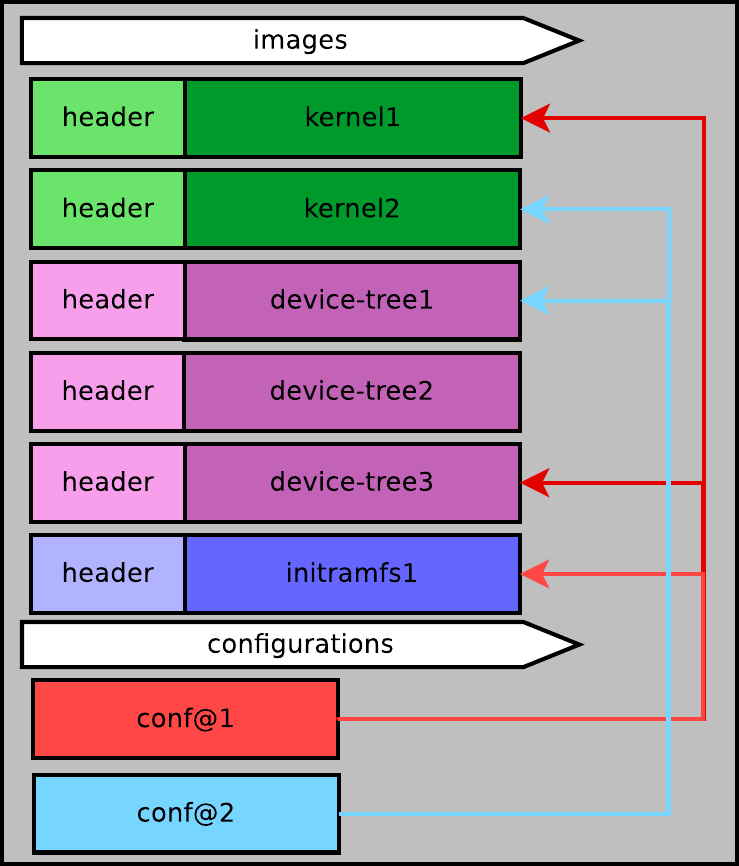
\includegraphics[height=0.9\textheight]{images/fitImage.png}
\end{center}
\end{frame}

%
%\begin{multicols}{2}
%[
%\section{First Section}
%All human things are subject to decay. And when fate summons, Monarchs must obey.
%]
%\columnbreak
%\end{multicols}


% *******************************
% **** Construction fitImage ****
% *******************************

\section{Construire fitImage}

\begin{frame}
\begin{center}
\huge{Construire une fitImage}
\end{center}
\end{frame}

\begin{frame}
Étapes:
\begin{center}
\begin{itemize}
	\item Générer une paire de clé (ex: avec openssl)
	\item Choisir son algo de signature
	\item Créer un descripteur \texttt{fitImage.its}
	\item Signer avec \texttt{mkimage}
\end{itemize}
\end{center}
\end{frame}

% **** Type de signature ****

\subsection{Type de signature}

\begin{frame}
\begin{center}
\large{Comment choisir son algo de signature ?}
\end{center}
\end{frame}

\begin{frame}[fragile]
Avant novembre 2016:
Plusieurs types de signature sont disponible dans U-Boot.\newline
\texttt{common/image-sig.c}
\begin{lstlisting}[style=shell,basicstyle=\tiny\ttfamily\color{white}]
struct image_sig_algo image_sig_algos[] = {
    {
        "sha1,rsa2048",
        rsa_sign,
        rsa_add_verify_data,
        rsa_verify,
        &checksum_algos[0],
    },
    {
        "sha256,rsa2048",
        rsa_sign,
        rsa_add_verify_data,
        rsa_verify,
        &checksum_algos[1],
    },
    {
        "sha256,rsa4096",
        rsa_sign,
        rsa_add_verify_data,
        rsa_verify,
        &checksum_algos[2],
    }

};
\end{lstlisting}
\end{frame}

\begin{frame}[fragile]
Après novembre 2016:

\begin{lstlisting}[language=C,basicstyle=\tiny\ttfamily\color{white}]
struct crypto_algo *image_get_crypto_algo(const char *full_name);
\end{lstlisting}
{\setlength\multicolsep{0pt}
\begin{multicols}{2}
\begin{lstlisting}[style=shell,basicstyle=\tiny\ttfamily\color{white}]
struct checksum_algo checksum_algos[] = {
	{
		.name = "sha1",
		.checksum_len = SHA1_SUM_LEN,
		.der_len = SHA1_DER_LEN,
		.der_prefix = sha1_der_prefix,
#if IMAGE_ENABLE_SIGN
		.calculate_sign = EVP_sha1,
#endif
		.calculate = hash_calculate,
	},
	{
		.name = "sha256",
		.checksum_len = SHA256_SUM_LEN,
		.der_len = SHA256_DER_LEN,
		.der_prefix = sha256_der_prefix,
#if IMAGE_ENABLE_SIGN
		.calculate_sign = EVP_sha256,
#endif
		.calculate = hash_calculate,
	}

};
\end{lstlisting}
\columnbreak
\begin{lstlisting}[style=shell,basicstyle=\tiny\ttfamily\color{white}]
struct crypto_algo crypto_algos[] = {
	{
		.name = "rsa2048",
		.key_len = RSA2048_BYTES,
		.sign = rsa_sign,
		.add_verify_data = rsa_add_verify_data,
		.verify = rsa_verify,
	},
	{
		.name = "rsa4096",
		.key_len = RSA4096_BYTES,
		.sign = rsa_sign,
		.add_verify_data = rsa_add_verify_data,
		.verify = rsa_verify,
	}

};
\end{lstlisting}
\end{multicols}
}
\end{frame}

%**** Descripteur de fitImage *****

\subsection{Descripteur \texttt{fitImage}}

\begin{frame}
\begin{center}
\large{Créer un descripteur de contenue de \texttt{fitImage}}
\end{center}
\end{frame}

\begin{frame}[fragile]
% Prevent first column disapear
\begin{lstlisting}[style=shell,basicstyle=\tiny\ttfamily\color{white}]
KERNEL=/path/to/zImage
KEYNAME=my_key
DTB=/path/to/.dtb
\end{lstlisting}
\begin{columns}
\begin{column}{0.5\textwidth}
\texttt{fitImage.its}
\begin{lstlisting}[style=shell,basicstyle=\tiny\ttfamily\color{white}]
/dts-v1/;

/ {
	description = "fitImage for sign Kernel image and DTB";
	#address-cells = <1>;

	images {
		kernel@1 {
			description = "Linux Kenel";
			data = /incbin/("%KERNEL%");
			type = "kernel";
			arch = "arm";
			os = "linux";
			compression = "none";
			load = <0x12000000>;
			entry = <0x12000000>;
			signature@1 {
				algo = "sha256,rsa4096";
				key-name-hint = "%KEYNAME%";
			};
		};
\end{lstlisting}
\end{column}
\begin{column}{0.5\textwidth}
\begin{lstlisting}[style=shell,basicstyle=\tiny\ttfamily\color{white}]
		fdt@1 {
			description = "Devicetree";
			data = /incbin/("%DTB%");
			type = "flat_dt";
			arch = "arm";
			compression = "none";
			load = <0x18000000>;
			entry = <0x18000000>;
			signature@1 {
				algo = "sha256,rsa4096";
				key-name-hint = "%KEYNAME%";
			};
		};
	};
	configurations {
		default = "conf@1";
		conf@1 {
			kernel = "kernel@1";
			fdt = "fdt@1";
		};
	};
};
\end{lstlisting}
\end{column}
\end{columns}
\end{frame}


% **** Signer les images ****

\subsection{Signer les images}

\begin{frame}
\begin{center}
\large{Signer les images avec \texttt{mkimage}}
\end{center}
\end{frame}

\begin{frame}[fragile]
Il faut l'ajouter avec \texttt{mkimage}:
\begin{description}
\item[-D <dtc options>] Fournie les options du compilateur de device tree utilisé pour créer l'image.
\item[-k <key\_directory>] Spécifie le répertoire contenant les clés pour signer. Il doit contenir la clé privé <name>.key et le certificat <name>.cert (contenant la clé public) utilisé pour la vérification.
\item[-K <key\_destination>] Spécifie le binaire compilier du device tree (.dtb) où écrire la clé public.
\item[-r] Spécifie la \texttt{fitImage}.
\end{description}
\end{frame}

\begin{frame}[fragile]
Pour signer:
\begin{lstlisting}[style=shell]
$ mkimage -D "-I dts -O dtb -p 4096" -f /path/to/fitImage.its -K /path/to/u-boot_pubkey.dtb -k /path/to/ -r fitImage
\end{lstlisting}
Cette opération doit être effectué avant la compilation d'\texttt{U-Boot}, car cette même commande permet d'inclure la clé public dans le dtb.
\vfill
l'option \texttt{-D "-I dts -O dtb -p 4096"} sera explique après.
\end{frame}


% **************************************
% **** Ajouter la clé dans U-Boot ****
% **************************************

\section{Ajouter la clé dans U-Boot}

\begin{frame}
\begin{center}
\huge{Ajouter la clé dans U-Boot}
\end{center}
\end{frame}

\begin{frame}
Étapes:
\begin{center}
\begin{itemize}
	\item Créer un \texttt{external dtb}
	\item Ajouter la clé à un \texttt{external dtb}
	\item Ajouter l'\texttt{external dtb} à la compilation d'Uboot
\end{itemize}
\end{center}
\end{frame}

%**** Créer un external dtb ****

\subsection{Créer un \texttt{external dtb}}

\begin{frame}
\begin{center}
\large{Créer un \texttt{external dtb}}
\end{center}
\end{frame}

\begin{frame}[fragile]
Créer un \texttt{devicetree}\footnote{arborescence de périphériques} spécifique.
\texttt{u-boot\_pubkey.dts}
\begin{lstlisting}
/dts-v1/;
/ {
	model = "Keys";
	compatible ="vendor,board";
	signature {
		key-%KEYNAME% {
			required = "image";
			algo = "sha256,rsa4096";
			key-name-hint = "%KEYNAME%";
		};
	};
};
\end{lstlisting}
\end{frame}

\begin{frame}[fragile]
Pour le générer le dtb:
\begin{lstlisting}[style=shell]
$ dtc -p 4096 $(@D)/u-boot_pubkey.dts -O dtb -o $(@D)/u-boot_pubkey.dtb
\end{lstlisting}
l'option \texttt{-p 4096} pernet de réserver un espace pour accueillir la clé.\newline
\newline
La clé n'est pas présente:
\begin{lstlisting}[style=shell]
$ cat u-boot_pubkey.dtb
vendor,board signature key-my_key image sha256,rsa4096 my_key modelcompatiblerequiredalgokey-name-hint
\end{lstlisting}
\end{frame}

%**** Ajouter la clé à l'external dtb ****

\subsection{Ajouter la clé à l'\texttt{external dtb}}

\begin{frame}
\begin{center}
\large{Ajouter la clé à l'\texttt{external dtb}}
\end{center}
\end{frame}

\begin{frame}[fragile]
Pour y ajouter la clé public il faut utiliser la commande de création de \texttt{fitImage}:
\begin{lstlisting}[style=shell]
$ mkimage -D "-I dts -O dtb -p 4096" -f /path/to/fitImage.its -K /path/to/u-boot_pubkey.dtb -k /path/to/ -r fitImage
\end{lstlisting}
Ce qui donne:
\begin{lstlisting}[style=shell]
$ cat u-boot_pubkey.dtb
vendor,board signature key-my_key
[...]
image sha256,rsa4096 my_key modelcompatiblerequiredalgokey-name-hintrsa,num-bitrsa,n0-inversersa,exponentrsa,modulusra,r-squaredsquared
\end{lstlisting}     
\end{frame}

%**** Ajouter l'external dtb à la compilation d'U-Boot ****

\subsection{Ajouter l'\texttt{external dtb} à la compilation d'U-Boot}

\begin{frame}
\begin{center}
\large{Ajouter l'\texttt{external dtb} à la compilation d'U-Boot}
\end{center}
\end{frame}

\begin{frame}[fragile]
Pour ajouter ce DTB spécifique dans U-Boot (même s'il n'y a pas de dtb) il faut utiliser l'option \texttt{EXT\_DTB} de make:
\begin{lstlisting}[style=shell]
$ make CROSS_COMPILE=arm-linux-gnueabihf- EXT_DTB=u-boot_pubkey.dtb
\end{lstlisting}
\end{frame}

%**** Exemple: logs U-Boot ****

\subsection{Exemple: logs U-Boot}

\begin{frame}
\begin{center}
\large{Exemple: logs U-boot}
\end{center}
\end{frame}

\begin{frame}[fragile]
\begin{lstlisting}[style=shell,basicstyle=\tiny\ttfamily\color{white}]
=> bootm 0x15000000 #or bootm 0x15000000#conf@1 since conf@1 is the default
## Loading kernel from FIT Image at 15000000 ...
   Using'conf@1'configuration
   Verifying Hash Integrity ... OK
   Trying'kernel@1'kernel subimage
     Description:  Linux kernel
     Type:         Kernel Image
     Compression:  uncompressed
     Data Start:   0x150000e4
     Data Size:    7010496 Bytes=6.7 MiB
     Architecture: ARM
     OS:           Linux
     Load Address: 0x12000000
     Entry Point:  0x12000000
     Hash algo:    sha256
     Hash value:   7d1fb52f2b8d1a98d555e01bc34d11550304fc26
     Sign algo:    sha256,rsa4096:my_key
     Sign value:   [redacted]
   Verifying Hash Integrity ... sha256,rsa4096:my_key+ sha256+ OK
## Loading fdt from FIT Image at 15000000 ...
   Using 'conf@1' configuration
   Trying 'fdt@1' fdt subimage
[...]
   Verifying Hash Integrity ... sha256,rsa4096:my_key+ sha256+ OK
   Booting using the fdt blob at 0x156afd40
   Loading Kernel Image ... OK
   Loading Device Tree to 1fff2000, end 1ffff1ed ... OK

Starting kernel...
\end{lstlisting}
\end{frame}


% *******************************
% ****     PRÉSENTATION      ****
% *******************************

%\subsection{uboot}
%\begin{frame}[fragile]
%J'ai rajouté quelques config dans buildroot.
%\begin{lstlisting}[style=shell]
%BR2_PACKAGE_UBOOT_TOOLS_FIT_SUPPORT=y
%BR2_PACKAGE_UBOOT_TOOLS_FIT_SIGNATURE_SUPPORT=y
%BR2_PACKAGE_HOST_UBOOT_TOOLS=y
%BR2_PACKAGE_HOST_UBOOT_TOOLS_FIT_SUPPORT=y
%BR2_PACKAGE_HOST_UBOOT_TOOLS_FIT_SIGNATURE_SUPPORT=y
%
%BR2_TARGET_UBOOT_NEEDS_OPENSSL=y
%
%BR2_TARGET_UBOOT_SIGN_FITIMAGE=y
%BR2_TARGET_UBOOT_ITS="$(CONFIG_DIR)/board/eolane/modx6/fitImage.its"
%BR2_TARGET_UBOOT_SIGN_DTS="$(CONFIG_DIR)/board/eolane/modx6/u-boot_pubkey.dts"
%BR2_TARGET_UBOOT_KEY_NAME="my_key"
%BR2_TARGET_UBOOT_KEY_SERVER="bep@hgweb:/home/apache/distribution/keys/"
%\end{lstlisting}
%\end{frame}
%
%\begin{frame}[fragile]{Vérification de la signature}
%il est possible de tester la signature d'une image avec:
%\begin{lstlisting}[style=shell]
%fit_check_sign -f output/images/fitImage -k u-boot_pubkey.dtb
%\end{lstlisting}
%dans \texttt{./output/build/host-uboot-tools-2017.07/tools/fit\_check\_sign}
%\end{frame}
%


% *******************************
% ****     PRÉSENTATION      ****
% *******************************
\section{Gestion dans Buildroot}

\begin{frame}
\begin{center}
\huge{Gestion dans Buildroot}
\end{center}
\end{frame}

\begin{frame}
Étapes:
\begin{itemize}
\item Rendre automatique la récupération des clés et la completion des descripteurs (\texttt{.its}, \texttt{.dtb}).
\item Ajouter la clé à l'\texttt{external dtb} pour compiler U-Boot.
\item Signer les images contenues dans la \texttt{fitImage}.
\end{itemize}
\end{frame}

\begin{frame}[fragile]
\begin{lstlisting}[language=diff,basicstyle=\fontsize{5}{5}\selectfont\ttfamily\color{white}]
--- a/boot/uboot/Config.in
+++ b/boot/uboot/Config.in
@@ -167,6 +167,38 @@ config BR2_TARGET_UBOOT_NEEDS_OPENSSL
 	  typically the case when the board configuration has
 	  CONFIG_FIT_SIGNATURE enabled.
 
+if BR2_TARGET_UBOOT_NEEDS_OPENSSL
+
+config BR2_TARGET_UBOOT_SIGN_FITIMAGE
+	bool "Sign fitImage"
+	depends on BR2_PACKAGE_HOST_UBOOT_TOOLS_FIT_SIGNATURE_SUPPORT
+	help
+	  Sign fitImage. This need external dtb for uboot, its file and openssl key.
+
+if BR2_TARGET_UBOOT_SIGN_FITIMAGE
+
+config BR2_TARGET_UBOOT_ITS
+	string "its file"
+	help
+	  its file need to have absolute path.
+
+config BR2_TARGET_UBOOT_SIGN_DTS
+	string "dts key file"
+	help
+	  dts file need to have absolute path. This will use as external dtb.
+
+config BR2_TARGET_UBOOT_KEY_NAME
+	string "Keys name"
+	help
+	  Name of public and private key
+
+config BR2_TARGET_UBOOT_KEY_SERVER
+	string "Keys server"
+	help
+	  Server adress to get keys
+endif
+endif
+
 config BR2_TARGET_UBOOT_NEEDS_LZOP
 	bool "U-Boot needs lzop"
 	help
\end{lstlisting}
\end{frame}

\begin{frame}[fragile]
\begin{lstlisting}[language=diff,basicstyle=\fontsize{5}{5}\selectfont\ttfamily\color{white}]
--- a/boot/uboot/uboot.mk
+++ b/boot/uboot/uboot.mk
@@ -246,6 +246,30 @@ define UBOOT_HELP_CMDS
 
+# Sign fitImage
+ifneq ($(call qstrip,$(BR2_TARGET_UBOOT_SIGN_FITIMAGE)),)
+UBOOT_MAKE_OPTS += EXT_DTB="$(@D)/u-boot_pubkey.dtb"
+endif
+
+ifneq ($(BR2_TARGET_UBOOT_SIGN_FITIMAGE),)
+UBOOT_ITS_PATH = $(call qstrip,$(BR2_TARGET_UBOOT_ITS))
+UBOOT_EXT_DTS = $(call qstrip,$(BR2_TARGET_UBOOT_SIGN_DTS))
+UBOOT_KEY_NAME = $(call qstrip,$(BR2_TARGET_UBOOT_KEY_NAME))
+UBOOT_KEY_SERVER = $(call qstrip,$(BR2_TARGET_UBOOT_KEY_SERVER))
+DTS_NAME = $(call qstrip,$(BR2_LINUX_KERNEL_INTREE_DTS_NAME))
+define UBOOT_SIGN_FITIMAGE
+	wget $(UBOOT_KEY_SERVER)/$(UBOOT_KEY_NAME).key -O $(@D)/$(UBOOT_KEY_NAME).key
+	wget $(UBOOT_KEY_SERVER)/$(UBOOT_KEY_NAME).crt -O $(@D)/$(UBOOT_KEY_NAME).crt
+	sed -e "s|%KERNEL%|$(BINARIES_DIR)/zImage|" $(UBOOT_ITS_PATH) > $(@D)/fitImage.its
+	sed -e "s|%DTB%|$(BINARIES_DIR)/$(DTS_NAME).dtb|" -i $(@D)/fitImage.its
+	sed -e "s|%KEYNAME%|$(UBOOT_KEY_NAME)|" -i $(@D)/fitImage.its
+	sed -e "s|%KEYNAME%|$(UBOOT_KEY_NAME)|" $(UBOOT_EXT_DTS) > $(@D)/u-boot_pubkey.dts
+	$(HOST_DIR)/bin/dtc -p 4096 $(@D)/u-boot_pubkey.dts -O dtb -o $(@D)/u-boot_pubkey.dtb
+	PATH=$(PATH):$(HOST_DIR)/bin $(HOST_DIR)/bin/mkimage -D "-I dts -O dtb -p 4096" -f $(@D)/fitImage.its -K $(@D)/u-boot_pubkey.dtb -k $(@D) -r $(BINARIES_DIR)/fitImage
+endef
+UBOOT_PRE_BUILD_HOOKS += UBOOT_SIGN_FITIMAGE
+endif
+
 UBOOT_CUSTOM_DTS_PATH = $(call qstrip,$(BR2_TARGET_UBOOT_CUSTOM_DTS_PATH))
 
 define UBOOT_BUILD_CMDS
@@ -329,6 +353,11 @@ endif
 
+define UBOOT_REMOVE_KEY
+	rm -f $(@D)/$(UBOOT_KEY_NAME).key $(@D)/$(UBOOT_KEY_NAME).crt $(@D)/$(UBOOT_KEY_NAME).pub
+endef
+UBOOT_POST_INSTALL_IMAGES_HOOKS += UBOOT_REMOVE_KEY
+
 define UBOOT_INSTALL_OMAP_IFT_IMAGE
 	cp -dpf $(@D)/$(UBOOT_BIN_IFT) $(BINARIES_DIR)/
 endf
\end{lstlisting}

\end{frame}


% *******************************
% ****     PRÉSENTATION      ****
% *******************************
\section*{Conclusion}

\subsection{Documentation}

\begin{frame}[fragile]
Documentation:
\begin{itemize}
\item \url{https://elinux.org/images/e/e0/Josserand-schulz-secure-boot.pdf}
\item \url{https://www.denx.de/wiki/pub/U-Boot/Documentation/multi_image_booting_scenarios.pdf}
\item \url{https://elinux.org/images/8/8a/Vasut--secure_and_flexible_boot_with_u-boot_bootloader.pdf}
\end{itemize}
\end{frame}

\subsection{Questions}

\begin{frame}
\begin{center}
\begin{huge}
Des questions ?
\end{huge}
\end{center}
\begin{center}
\textcolor{gray}{\tiny{Enfin je vais essayer de répondre...}}
\end{center}
\center{\url{mickael@tansorier.fr}}
\vfill
\center{\textcolor{gray}{\tiny{GNU Free Documentation License, Version 1.3}}}
\end{frame}

\end{document}
